\chapter{Evaluation}
\label{ch:evaluation}
The evaluation chapter describes the experiment setup and the results.

\section{Experiment Setup}

The experiment setup consists of a client, a web server and a search engine.
Figure \ref{fig:experiment-setup} illustrates the experiment setup.
The client was a NodeJS script sending requests to the web server.

\begin{figure}[h!]
  \centering \includegraphics[width=0.9\linewidth]{img/experiment_setup.png}
  \caption{Experiment setup}
  \label{fig:experiment-setup}
\end{figure}

Elasticsearch's configuration was set to default settings,
except the memory heap size was changed to 4GB to make sure the search engine had sufficient memory.

\subsection{Hardware}
The experiment were conducted on a desktop computer with the specification described in table \ref{tbl:hardware}.

\begin{table}[h]
    \centering
    \begin{tabular}{c|c}
      \textbf{Component} & \textbf{Model} \\ \hline
      CPU       & Intel Core i5           \\ \hline
      RAM       & 16 GB                   \\ \hline
      SSD       & 256 GB                  \\ \hline
    \end{tabular}
    \caption{Hardware components of the computer running the experiments}
    \label{tbl:hardware}
\end{table}

\section{Result}
Measuring document relevance from users were never done as the main focus was latency and scaleability.

Latency was measure from the webserver recieved the request, to the server responded the user's request.
The round trip time from the webserver to the user is not taken into account.

As the web server and the search engine is on the same physical machine the round trip times are minimal.
However, in practice round trip times is often an important factor.

Figure \ref{fig:baseline} displays results from queries without query expansion.
The results without query expansion is used as a baseline,
to establish how much impact query expansion has on the respons times.

\begin{figure}
  \centering
  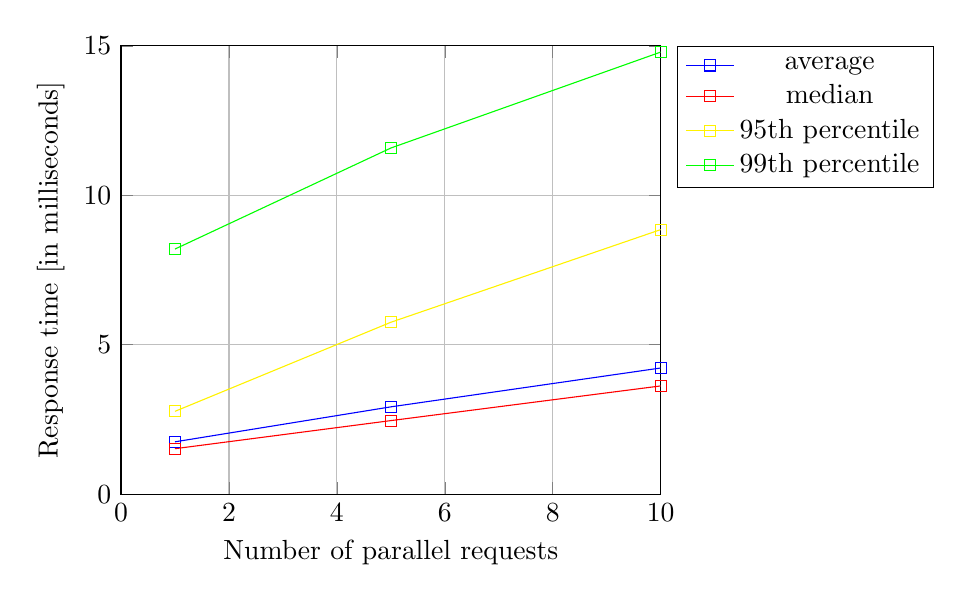
\begin{tikzpicture}[]
    \begin{axis}[
        xlabel={Number of parallel requests},
        ylabel={Response time [in milliseconds]},
        xmin=0, xmax=10,
        ymin=0, ymax=15,
        %legend pos=north west,
        grid=major,
        grid style=thin,
        legend pos=outer north east
      ]
        \addplot[
          color=blue,
          mark=square,
        ]
        coordinates {
          (1,   1.75)
          (5,   2.92)
          (10,  4.22)
        };
        \addlegendentry{average}

        \addplot[
          color=red,
          mark=square,
        ]
        coordinates {
          (1,   1.52)
          (5,   2.46)
          (10,  3.62)
        };
        \addlegendentry{median}

        \addplot[
          color=yellow,
          mark=square,
        ]
        coordinates {
          (1,   2.77)
          (5,   5.75)
          (10,  8.85)
        };
        \addlegendentry{95th percentile}

        \addplot[
          color=green,
          mark=square,
        ]
        coordinates {
          (1,   8.20)
          (5,   11.58)
          (10,  14.79)
        };
        \addlegendentry{99th percentile}
    \end{axis}
  \end{tikzpicture}
  \caption{Response time without query expansion}
  \label{fig:baseline}
\end{figure}

\begin{figure}
  \centering
  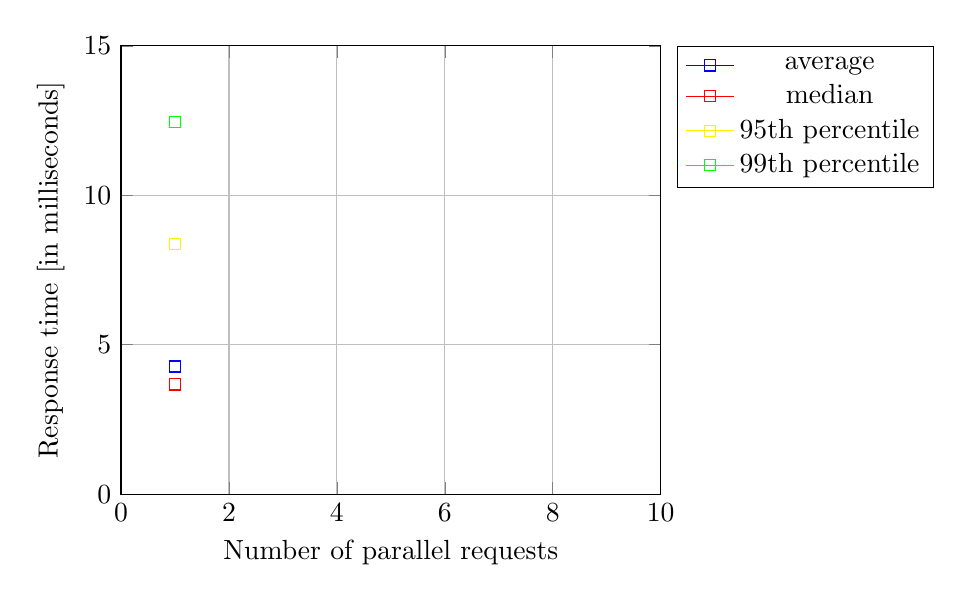
\begin{tikzpicture}[]
    \begin{axis}[
        xlabel={Number of parallel requests},
        ylabel={Response time [in milliseconds]},
        xmin=0, xmax=10,
        ymin=0, ymax=15,
        %legend pos=north west,
        grid=major,
        grid style=thin,
        legend pos=outer north east
      ]
        \addplot[
          color=blue,
          mark=square,
        ]
        coordinates {
          (1,   4.27)
        };
        \addlegendentry{average}

        \addplot[
          color=red,
          mark=square,
        ]
        coordinates {
          (1,   3.67)
        };
        \addlegendentry{median}

        \addplot[
          color=yellow,
          mark=square,
        ]
        coordinates {
          (1,   8.37)
        };
        \addlegendentry{95th percentile}

        \addplot[
          color=green,
          mark=square,
        ]
        coordinates {
          (1,   12.44)
        };
        \addlegendentry{99th percentile}
    \end{axis}
  \end{tikzpicture}
  \caption{Response time with query expansion}
  \label{fig:query-expansion}
\end{figure}


\centering
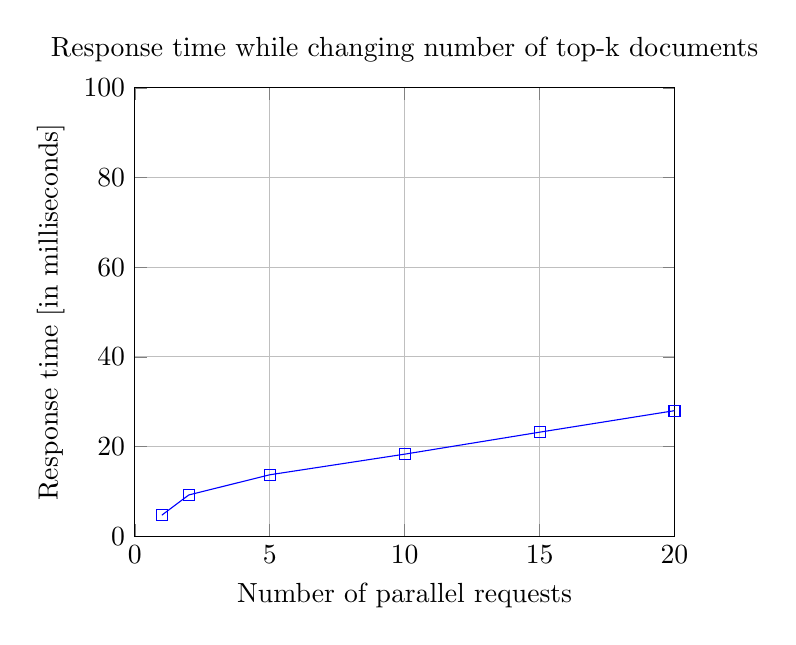
\begin{tikzpicture}[]
  \begin{axis}[
      title={Response time while changing number of top-k documents},
      xlabel={Number of parallel requests},
      ylabel={Response time [in milliseconds]},
      xmin=0, xmax=20,
      ymin=0, ymax=100,
      %legend pos=north west,
      grid=major,
      grid style=thin,
    ]
      \addplot[
        color=blue,
        mark=square,
      ]
      coordinates {
        (1,   4.7)
        (2,   9.2)
        (5,   13.7)
        (10,  18.3)
        (15,  23.2)
        (20,  28.0)
      };
  \end{axis}
  \label{fig:baseline}
\end{tikzpicture}

